\label{chap:pcb}
Wszystkie płytki stworzone na rzecz tej pracy magisterskiej zostały wykonane przez autorów pracy w warunkach domowych. W tym dodatku został opisany sposób wytwarzania płytek.

Do wykonania płytek PCB musimy posiadać maskę ścieżek które umieścimy na laminacie. Autorzy tej pracy magisterskiej użyli w tym celu programu Eagle w wersji edukacyjnej z której można korzystać za darmo. Po zaprojektowaniu schematu oraz layoutu płytki maska ścieżek była drukowana przy pomocy drukarki laserowej na papierze kredowym. Istotne jest dobre przygotowanie layoutu przed drukiem. Jeżeli ścieżki mają znajdować się na górnej stronie płytki, czyli po tej samej stronie po której będą umieszczane elementy elektroniczne, należy stworzyć odbicie lustrzane layoutu. Natomiast w przypadku ścieżek umiejscowionych na warstwie dolnej nie wykonujemy tego kroku. Bardzo przydatnym w tym momencie okazuje się jakiś znacznik na przykład tekst, który na wydruku powinien zawsze być odbiciem lustrzanym. Tak przygotowany layout drukujemy przy użyciu czarno--białej drukarki laserowej na papierze kredowym.

\begin{figure}[!ht]
 \centering
 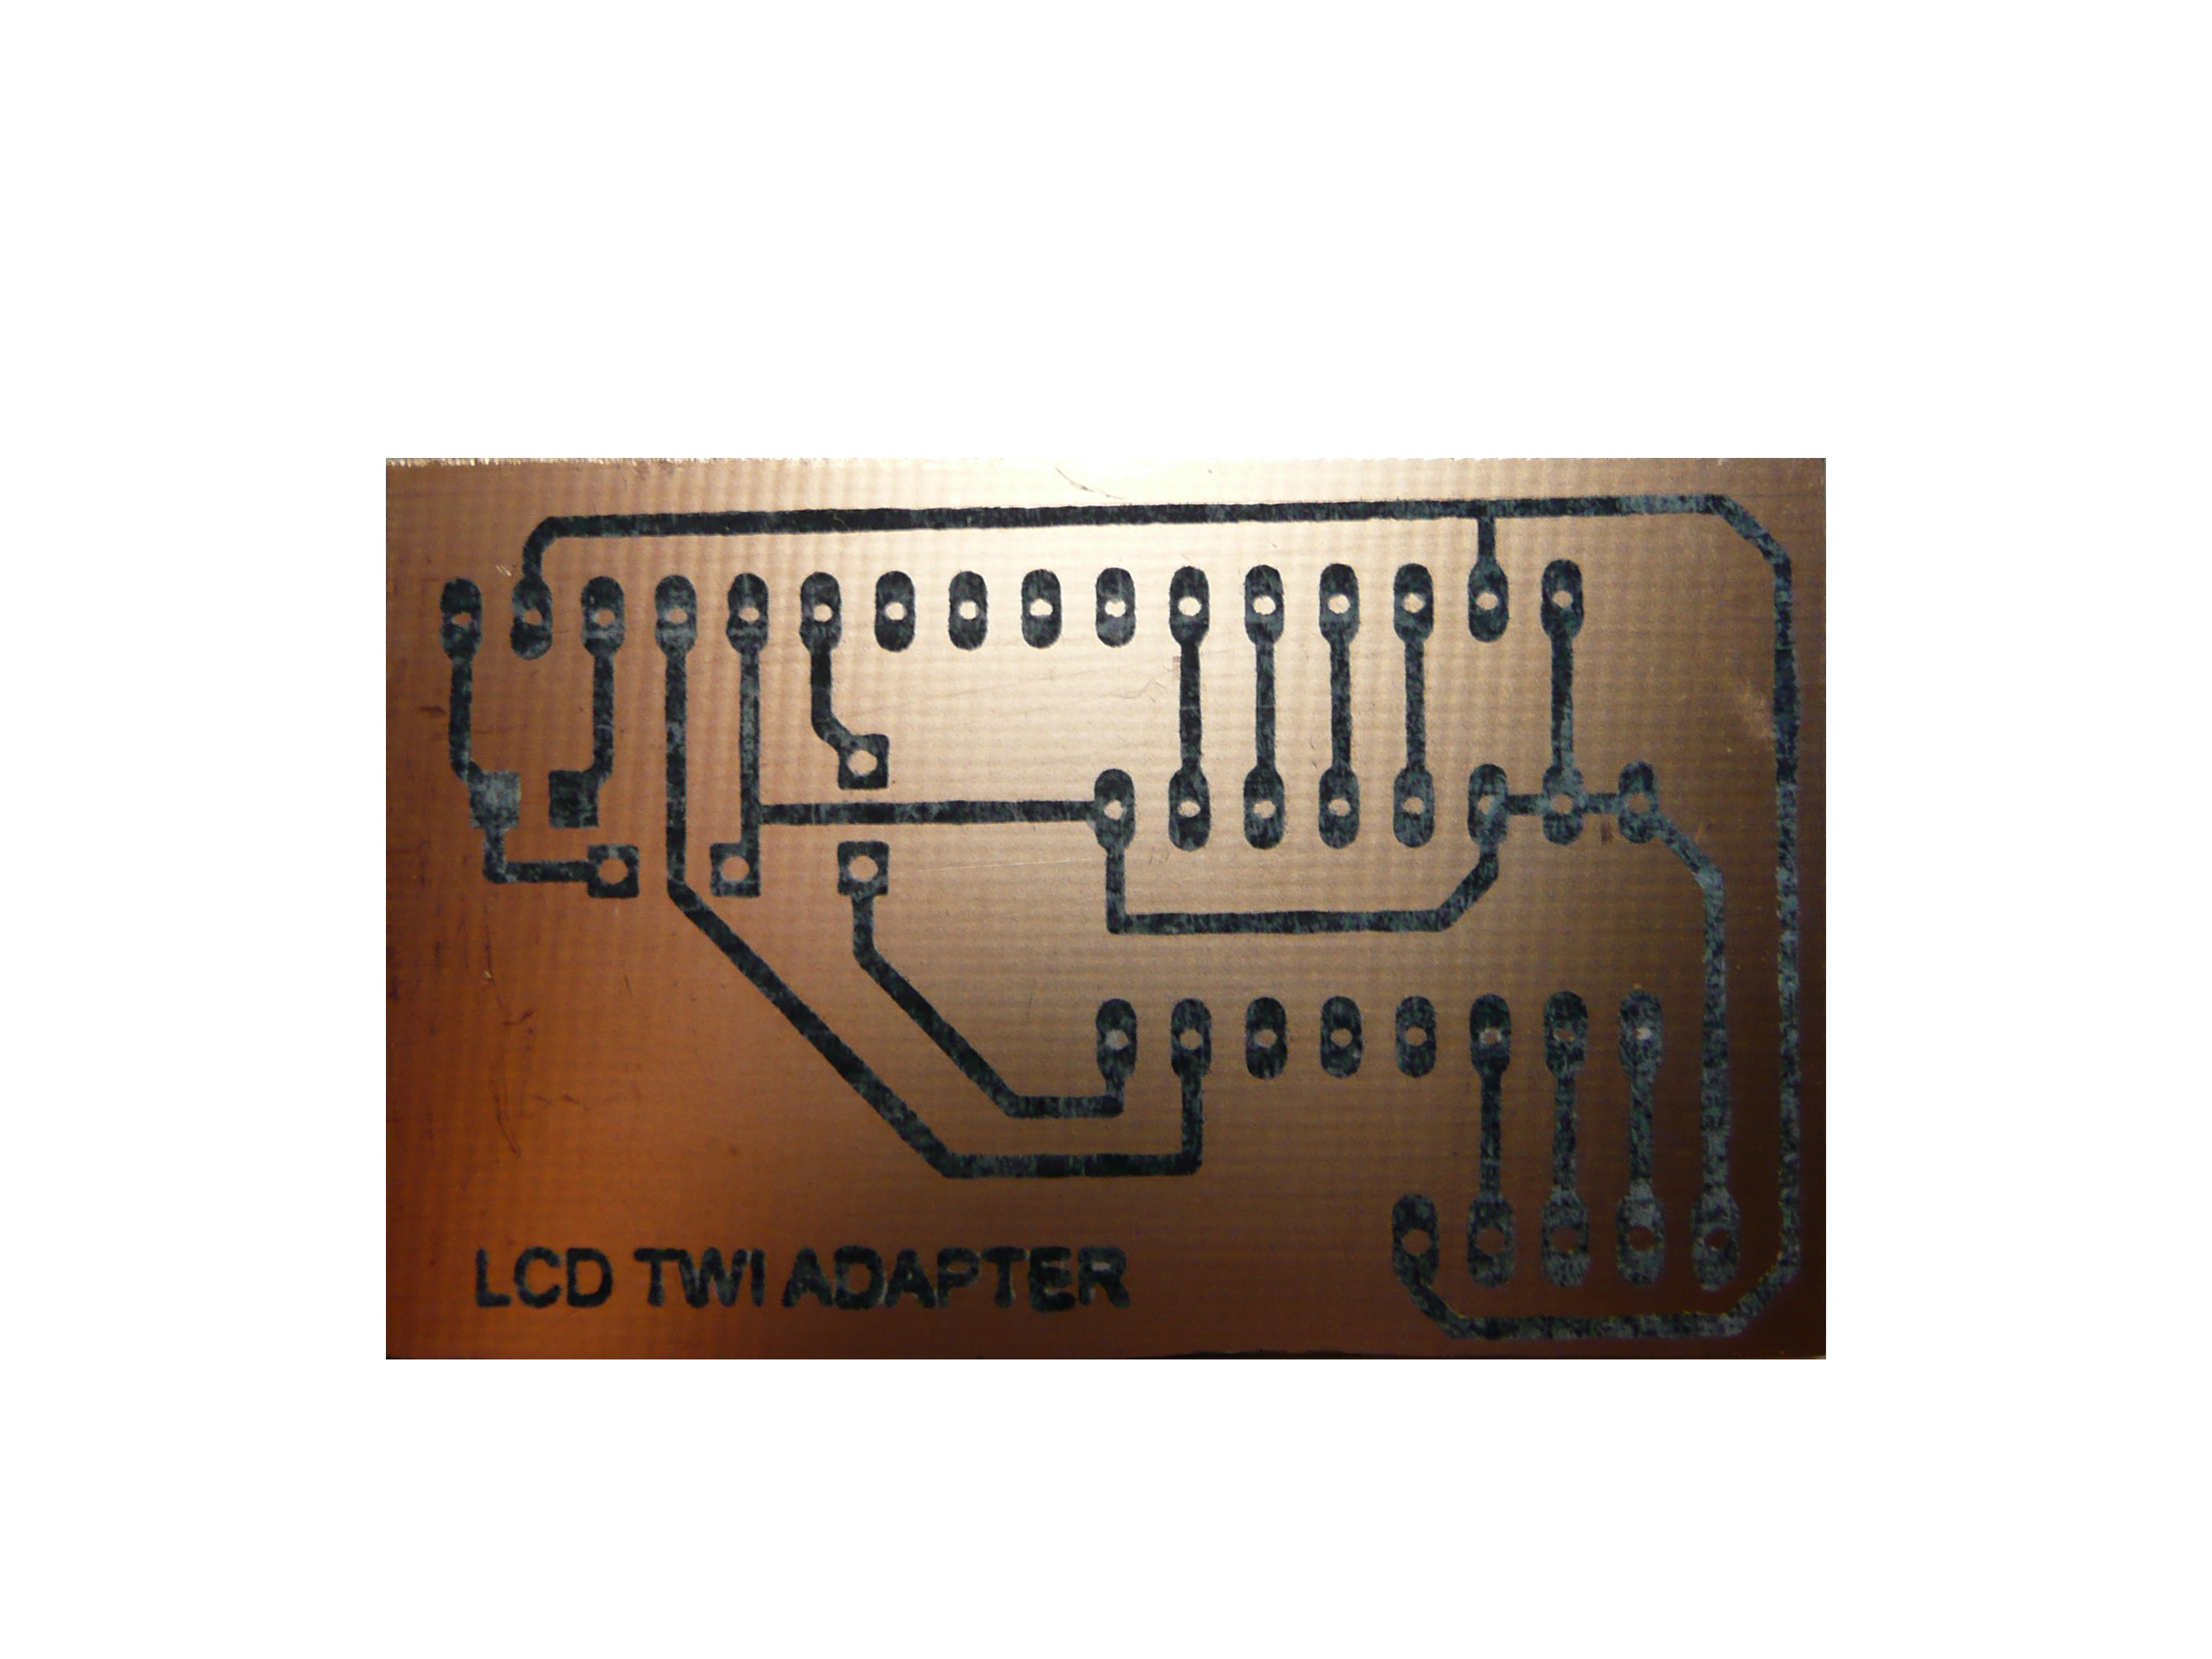
\includegraphics[height=50mm]{../images/appendix/toner.JPG}
 \caption{Płytka z naniesionym tonerem}
 \label{fig:PlytkaZTonerem}
\end{figure}

Po wydrukowaniu maski konieczne jest odpowiednie przygotowanie laminatu. W pierwszym kroku używamy papieru ściernego w celu zmatowienia laminatu. Następnie czyścimy laminat płynem do mycia naczyń w celu odtłuszczenia oraz osuszamy go. Po tych czynnościach możemy przystąpić do nakładania maski na laminat. Wycinamy jeden z wydrukowanych layoutów i przykładamy go zadrukowaną stroną do laminatu. Po tych przygotowaniach prasujemy całość żelazkiem rozgrzanym do temperatury $150^{\circ}C$ około 5 minut. Operacja ta powinna spowodować przeniesienie tonera z papieru na laminat. W celu usunięcia papieru kredowego wrzucamy płytkę do gorącej wody z dodatkiem proszku do prania. Papier powinien z łatwością się oderwać. Ewentualne przerwania w ścieżkach można poprawić markerem wodoodpornym. Jeżeli uzyskany efekt nie jest satysfakcjonujący powtarzamy całą operację usuwając wcześniej toner przy pomocy zmywacza do paznokci.

\begin{figure}[!ht]
 \centering
 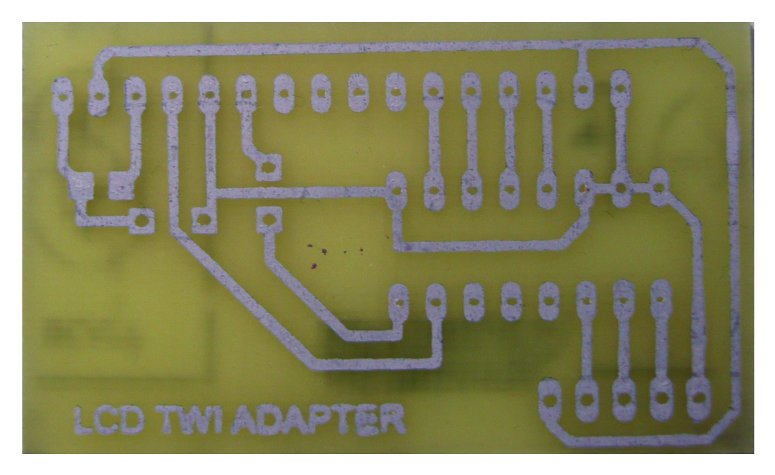
\includegraphics[height=50mm]{../images/appendix/wytrawiona.JPG}
 \caption{Wytrawiona płytka}
 \label{fig:WytrawionaPlytka}
\end{figure}

Istnieje wiele środków trawiących miedź. Autorzy tej pracy stosowali B327 czyli nadsiarczan sodowy. Ten środek trawiący działa najlepiej w temperaturze $50^{\circ}C$. W celu osiągnięcia optymalnych warunków do trawienia B327 należy rozcieńczyć w wodzie i umieścić w jakimś naczyniu. Następnie całość wkładamy do drugiego naczynia z gorącą wodą. W takich warunkach trawienie płytki nie powinno trwać dłużej niż 30 minut.

\begin{figure}[!ht]
 \centering
 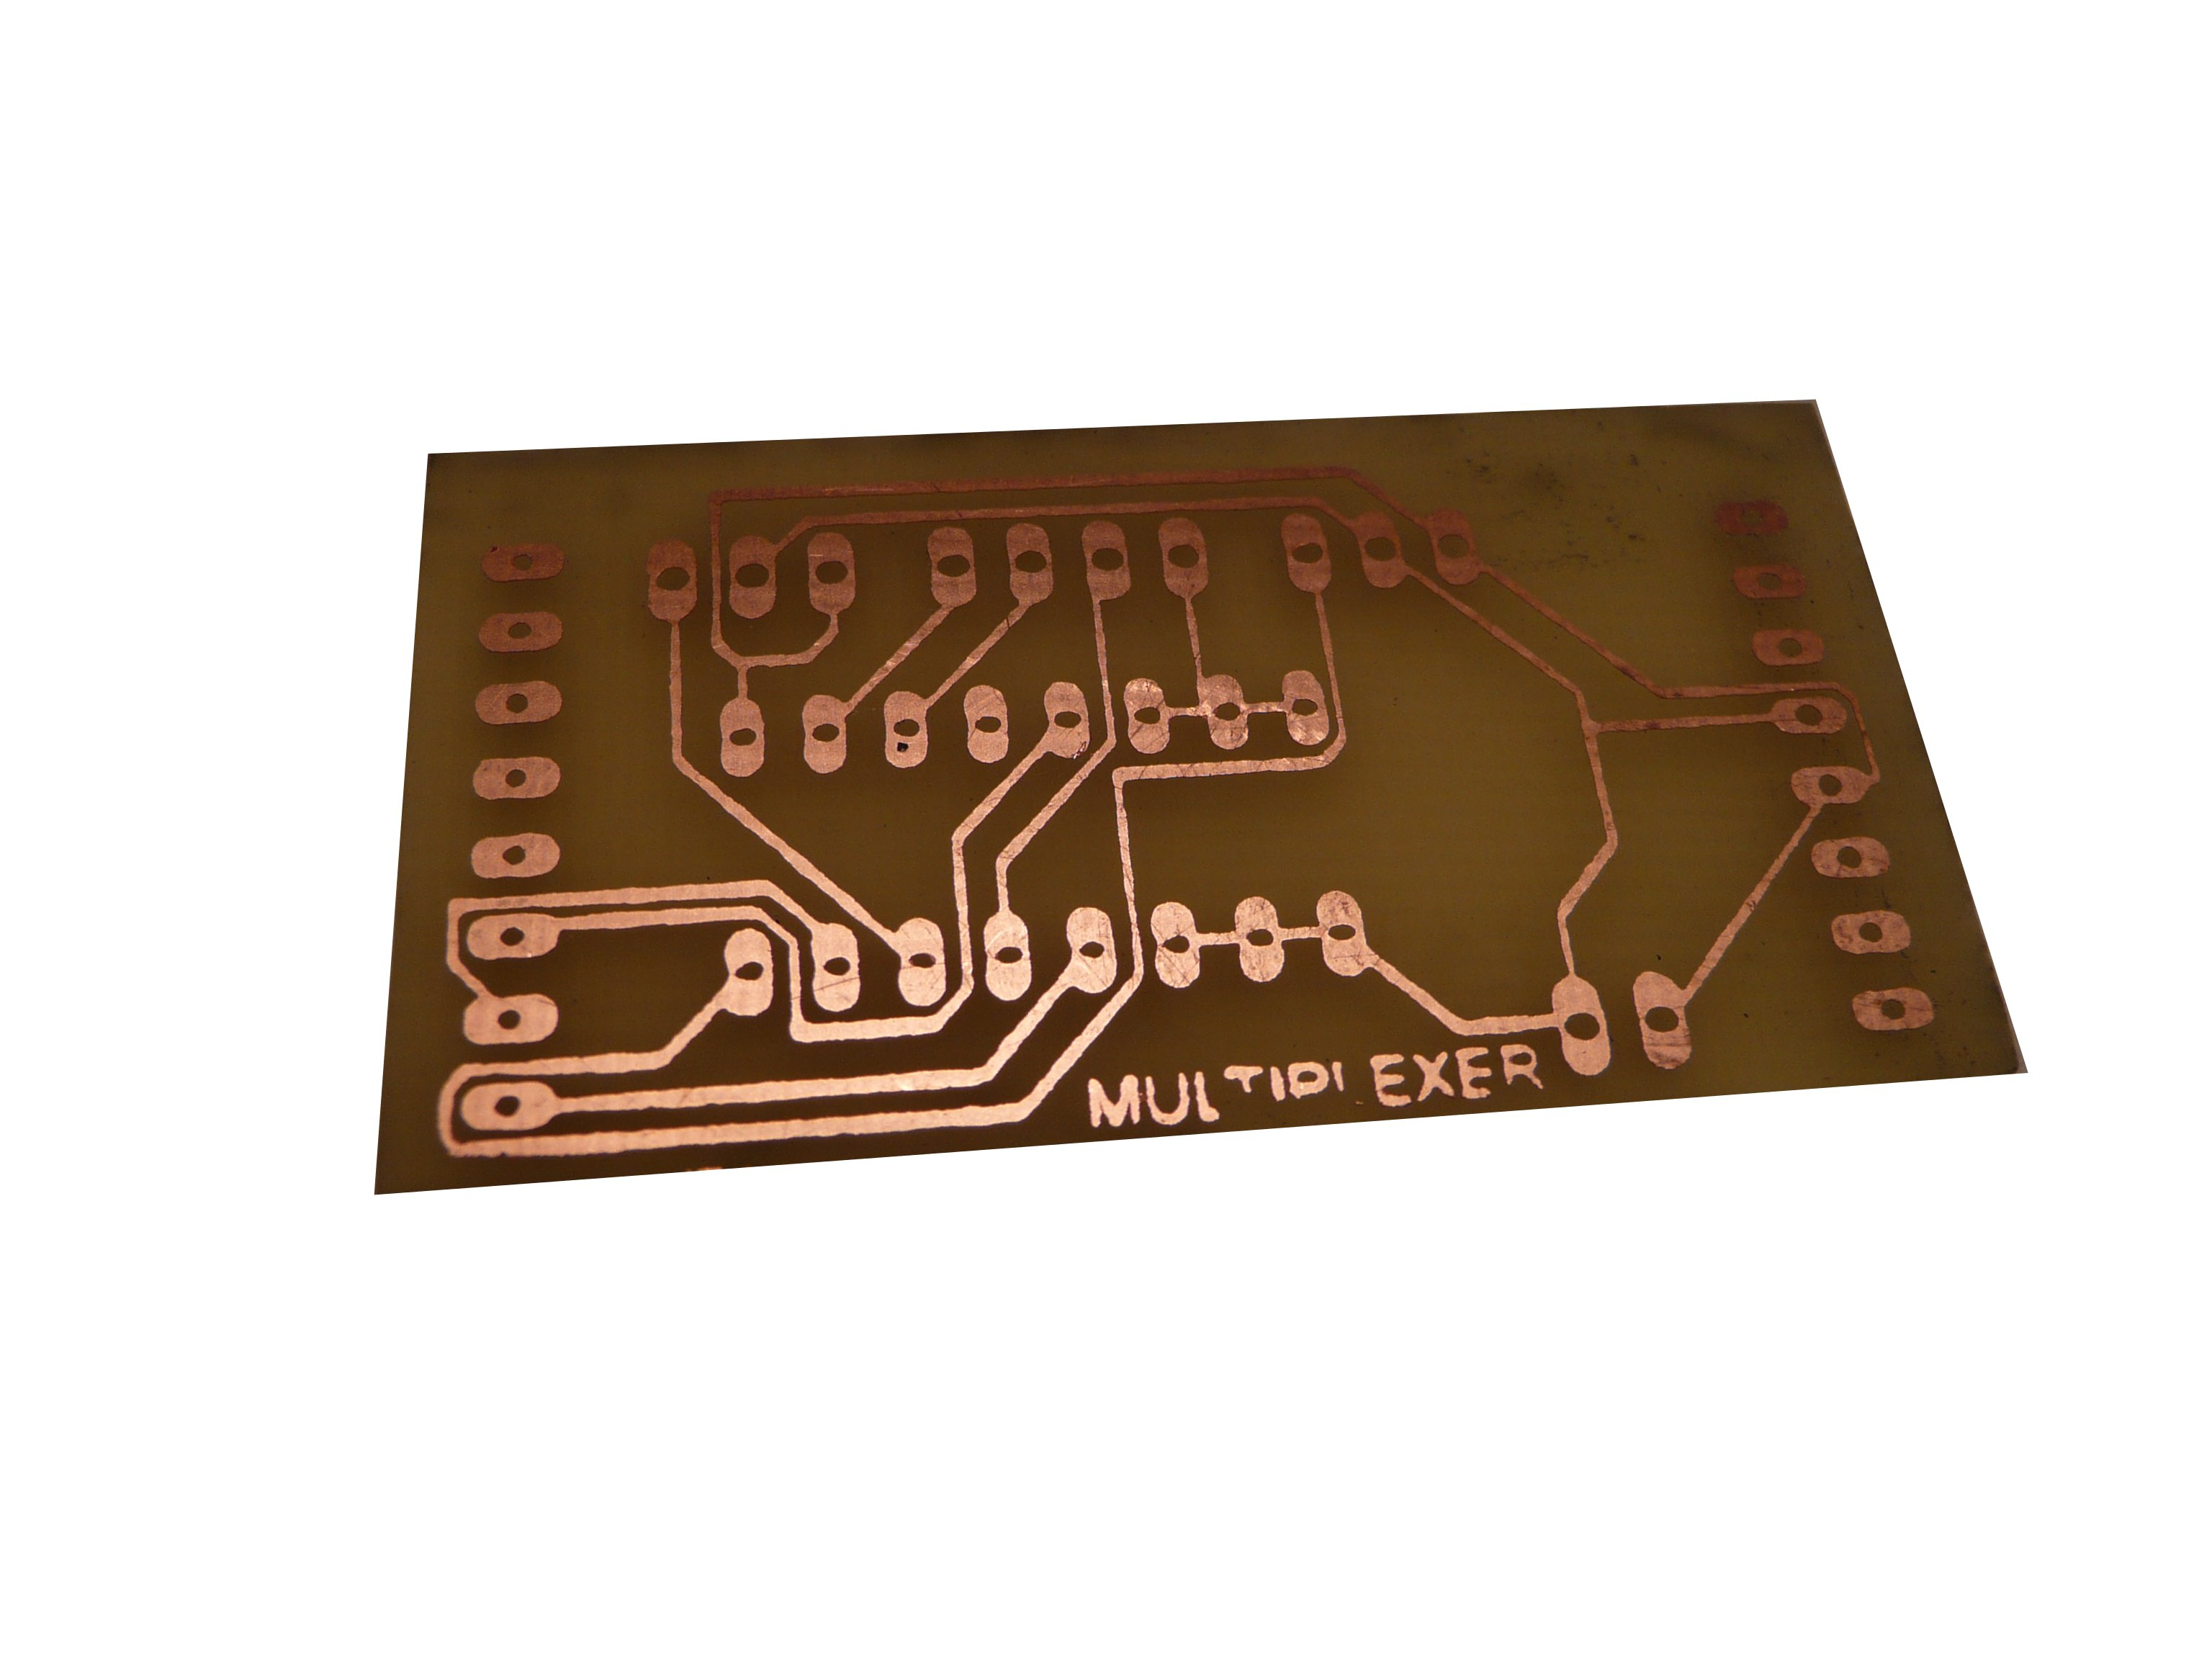
\includegraphics[height=50mm]{../images/appendix/gotowa.JPG}
 \caption{Gotowa płytka}
 \label{fig:GotowaPlytka}
\end{figure}

Po zakończeniu procesu trawienia należy usunąć toner przy pomocy zmywacza do paznokci i wywiercić otwory montażowe. Dzięki tej metodzie możemy tworzyć płytki z bardzo cienkimi ścieżkami wymagającymi precyzji, której nie da się osiągnąć przy ręcznym rysowaniu maski na laminacie. Kolejnymi atutami tej metody jest praktycznie zerowy koszt produkcji płytki oraz krótki czas realizacji.
